% Provenance (never printed): old terminale S material on past climates (ice cores,
% pollen, ocean sediments and oxygen isotopes, glacial-interglacial cycles, the
% astronomical rhythm told, climates of deep time), read from data. Owner (Sync 0/1):
% climate archive and proxy, ice core, glacial period, interglacial and glacial cycle,
% pollen analysis, Last Glacial Maximum. Recalled: glacier, ice sheet, ice age (Book 1,
% grade 8); the first look at the ice-core records (Book 1, grade 9); isotopes
% (physics); greenhouse gases (chemistry); the time scale (Book 1, grade 7). The
% delta notation of isotopes is Book 3's: isotope curves are read here as told,
% without a definition. The orbital theory of climate belongs to a university book:
% told here only. Physical science only, in the IPCC's calibrated words.
% Figures: figdata/grade-12/ice_age_records.py (tests/grade-12/test_ice_age_records.py).
\chapter{Leer los climas del pasado}\label{ch:g12:past-climates}

En el Domo~C, a \qty{3233}{m} de altitud sobre el inlandsis de la Antártida
Oriental, el aire tiene una media anual de unos \qty{-55}{\degreeCelsius}. Una
perforación hecha allí se detuvo a \qty{3260}{m} de profundidad, a unos
\qty{15}{m} de la roca que hay bajo el hielo. El hielo más profundo que subió
contiene diminutas burbujas de aire de unos \num{800000} años: una muestra de
la atmósfera de mucho antes de los primeros agricultores. Este capítulo
lee el clima del pasado en el hielo, en el lodo de los lagos y del fondo
oceánico, y en las rocas, y se pregunta qué nos dice sobre el presente.
% ledger: ipev:concordia, edc3:drilling, jouzel07:edc

\begin{omfigure}
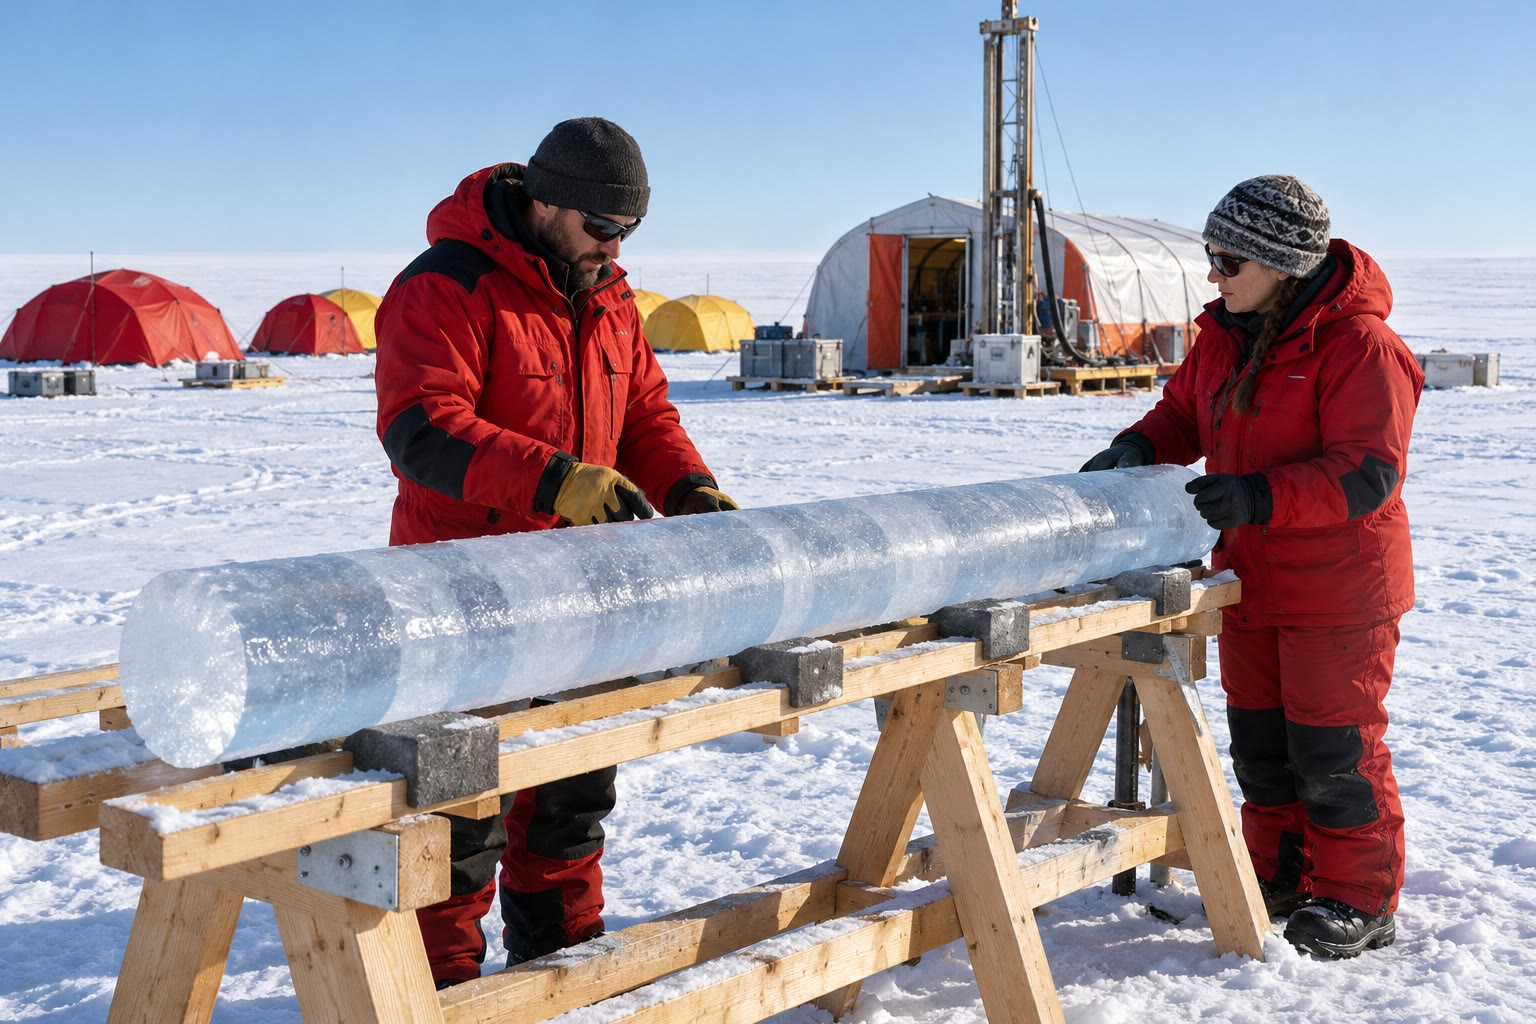
\includegraphics[width=0.56\linewidth]{images/book2/ai/g12-ice-coring-camp.jpg}

{\small Un campamento de perforación de hielo sobre un inlandsis polar: la sonda trabaja bajo la
torre y el refugio, y cada tramo de testigo se coloca, se registra y se
embala antes de viajar al laboratorio. Ilustración generada por IA.}
\end{omfigure}

\begin{recall}
Un glaciar es una masa de hielo que perdura de un año a otro y fluye por su
propio peso; un inlandsis cubre una gran parte de un continente; una glaciación es un
largo periodo frío en el que los inlandsis se extienden mucho más allá de los polos (Libro 1, año 8).
En los \omterm{def:g12:past-climates:ice-core}{testigos de hielo} de la Antártida, la nieve registra la temperatura del aire y las
burbujas guardan el propio aire, y los dos registros suben y bajan a la vez
(Libro 1, año 9). Los átomos de un mismo elemento pueden diferir en su número de
neutrones: estos isótopos se comportan igual en química pero difieren en masa (los
libros de física). El dióxido de carbono es un gas de efecto invernadero (los libros de química).
El periodo Cuaternario empezó hace 2.58 millones de años
(Libro 1, año 7).
\end{recall}
% ledger: ics:base.Quaternary (shared), nasaeo:o18 (snow poor in heavy isotopes)

\section{Archivos e indicadores indirectos}

Nadie midió la temperatura del aire hace \num{20000} años. Pero la
Tierra guardó registros sin proponérselo: capas de hielo y de lodo, conchas y troncos
de árboles, cada uno de los cuales cambió con el clima en el que se formó.

\begin{definition}[Archivo climático; indicador indirecto]\label{def:g12:past-climates:proxy}
Un \emph{archivo climático}\index{archivo climatico@archivo climático} es un material natural depositado
en capas, una tras otra, que guarda una huella del clima de la
época en que se formó: el hielo polar, los sedimentos de los lagos y del fondo
oceánico, los anillos de los árboles, los corales, los depósitos de las cuevas. Un \emph{indicador indirecto}\index{indicador indirecto} es una
magnitud medida en un archivo que sustituye a una variable climática que
no se midió: la proporción de isótopos pesados en la nieve antigua para la temperatura
del aire, la proporción de cada tipo de polen en el lodo de un lago para la vegetación
y, por tanto, para el clima.
\end{definition}
% ledger: ncei:proxy, ncei:pollen, nasaeo:o18

\begin{center}
\small
\begin{tabular}{|l|l|l|}
\hline
\textbf{archivo} & \textbf{\omterm{def:g12:past-climates:proxy}{indicador indirecto}} & \textbf{informa sobre} \\
\hline
hielo polar & isótopos pesados del hielo & temperatura del aire sobre el hielo \\
 & aire de las burbujas & dióxido de carbono, metano \\
sedimentos lacustres, turba & polen & vegetación y, de ahí, clima \\
sedimentos oceánicos & oxígeno 18 de las conchas & \shortstack[l]{volumen de hielo,\\temperatura del agua profunda} \\
anillos de los árboles & anchura de los anillos & condiciones de crecimiento, año a año \\
corales, depósitos de cuevas & isótopos, bandas de crecimiento & \shortstack[l]{temperatura del mar\\o del aire, lluvia} \\
\hline
\end{tabular}

\medskip
{\small Los principales \omterm{def:g12:past-climates:proxy}{archivos climáticos} y algunos de sus \omterm{def:g12:past-climates:proxy}{indicadores indirectos}.}
\end{center}
% ledger: ncei:proxy, nasaeo:o18

Todo \omterm{def:g12:past-climates:proxy}{indicador indirecto} necesita dos cosas antes de poder leerse. Necesita un \emph{reloj}:
la edad de cada capa, obtenida contando las capas anuales donde se ven,
por datación radiométrica (el \cref{ch:g12:age-of-the-earth}) o comparando el
registro con otro ya datado. Y necesita una \emph{calibración}: la
relación entre lo que se mide y la variable climática, establecida hoy, cuando
ambas pueden medirse a la vez.

\begin{method}[Leer un registro de un indicador indirecto]
\begin{enumerate}
  \item Identifica el archivo y el indicador: ¿qué se midió, y en qué?
  \item Averigua en qué sentido corre el tiempo en el eje, y en qué unidad;
        comprueba si el eje del indicador está invertido.
  \item Traduce el indicador: ¿un valor más alto significa más calor o más frío,
        más hielo o menos?
  \item Fíjate en la separación entre muestras: un registro cuyos puntos están
        separados \num{2000} años no puede mostrar un cambio que duró un siglo.
  \item Lee los valores en las fechas pedidas, o las medias en un intervalo,
        y calcula cambios y ritmos.
  \item Di lo que el registro muestra en su lugar y, solo después, si
        representa a toda la Tierra.
\end{enumerate}
\end{method}

\section{Testigos de hielo}

\begin{definition}[Testigo de hielo]\label{def:g12:past-climates:ice-core}
Un \emph{testigo de hielo}\index{testigo de hielo} es un cilindro de hielo extraído por perforación de un
inlandsis o de un glaciar. Su profundidad da la edad del hielo, tanto más antiguo cuanto más profundo;
el hielo registra la temperatura del aire en el que cayó su nieve, y sus
burbujas guardan muestras del aire de la época.
\end{definition}
% ledger: ncei:proxy, jouzel07:edc

La nieve recién caída es sobre todo aire. Enterrada bajo la nieve de los años siguientes, se
compacta en \emph{neviza}, una nieve compactada cuyos poros aún dejan pasar el aire.
A una densidad de unos 820 a \qty{830}{kg/m^3}, alcanzada entre 50 y \qty{120}{m}
de profundidad, los poros se cierran y el aire queda encerrado en burbujas. Por eso el hielo guarda dos
registros distintos. El aire de las burbujas es una muestra de la atmósfera, cuyo dióxido
de carbono y cuyo metano se miden en el laboratorio. El propio hielo guarda la
temperatura: las moléculas de agua que contienen un isótopo pesado (deuterio u
oxígeno 18) se condensan con más facilidad que las ligeras, de modo que cuanto más frío
es el aire en su camino hacia el polo, más pobre en isótopos pesados se vuelve la nieve.
% ledger: firn:close-off, nasaeo:o18

\begin{omfigure}
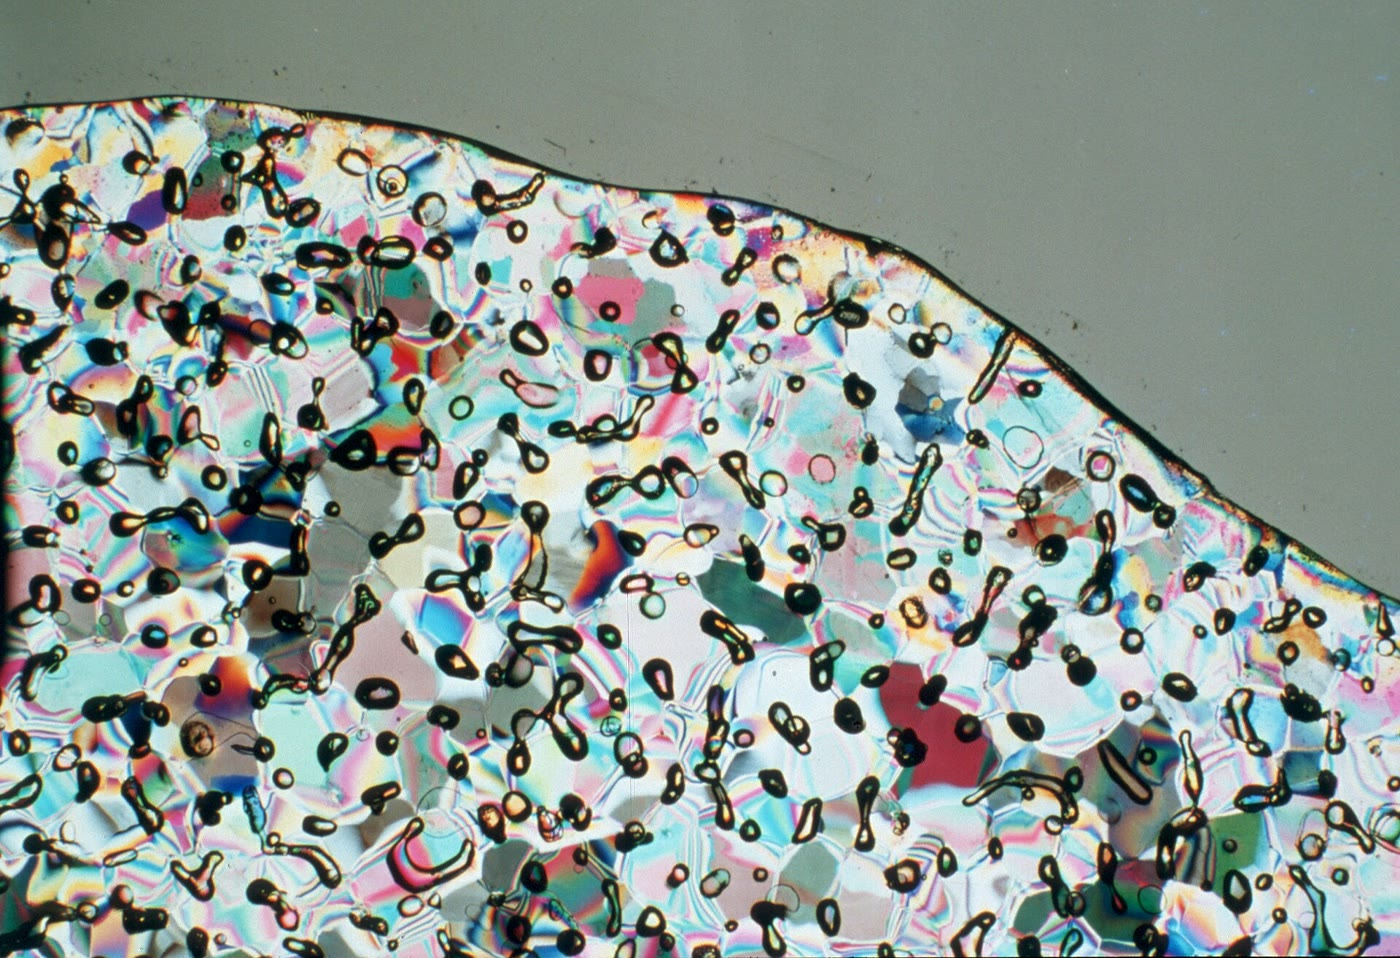
\includegraphics[width=0.50\linewidth]{images/book2/g12-ice-bubbles.jpg}

{\small Una lámina fina de hielo antártico vista con luz polarizada, que colorea
los cristales de hielo: los puntos oscuros son burbujas de aire atrapado. Fotografía de CSIRO
Atmospheric Research, CC~BY~3.0 (Wikimedia Commons).}
\end{omfigure}
% ledger: photo:g12-ice-bubbles

El deuterio del testigo del Domo~C se ha convertido en una temperatura sobre el
hielo, dada como un cambio respecto a la media de los últimos mil años. El
dióxido de carbono procede de las burbujas de varios testigos antárticos, reunidos
en un solo registro. Ambos se representan abajo sobre un mismo eje de tiempo.

\begin{omfigure}
\begin{tikzpicture}
\begin{axis}[omrecord, scale only axis, width=0.74\linewidth, height=4.8cm,
  xmin=0, xmax=800, x dir=reverse, ymin=-12, ymax=8, axis y line*=left,
  xtick={0,100,...,800}, ytick={-10,-5,0,5},
  xlabel={miles de años antes de 1950},
  ylabel={cambio de temperatura (\unit{\degreeCelsius})}]
% data:edc-jouzel, 2-kyr means (figdata/grade-12/ice_age_records.py)
\addplot[omWarm, line width=0.7pt] table[x=age_kyr, y=temp_C] {figdata/out/grade-12-ice_age_records-edc.dat};
\end{axis}
\begin{axis}[scale only axis, width=0.74\linewidth, height=4.8cm,
  xmin=0, xmax=800, x dir=reverse, ymin=60, ymax=320, axis y line*=right,
  axis x line=none, ytick={180,220,260,300}, ylabel={dióxido de carbono (ppm)},
  every axis label/.append style={font=\small}, tick label style={font=\small}]
% data:co2-bereiter, 2-kyr means
\addplot[black, line width=0.7pt] table[x=age_kyr, y=co2_ppm] {figdata/out/grade-12-ice_age_records-co2.dat};
\coordinate (lt) at (axis cs:560,70);
\coordinate (lc) at (axis cs:560,312);
\end{axis}
\node[font=\scriptsize, text=omWarm, anchor=south] at (lt) {temperatura en el Domo~C (escala izquierda)};
\node[font=\scriptsize, anchor=north] at (lc) {dióxido de carbono (escala derecha)};
\end{tikzpicture}

{\small Ochocientos mil años de hielo antártico, promediados por tramos de
\num{2000} años. Rojo: la temperatura en el Domo~C respecto a los últimos
mil años (Jouzel y otros, 2007); negro: el dióxido de carbono de las
burbujas (Bereiter y otros, 2015). El presente está a la derecha.}
\end{omfigure}
% ledger: data:edc-jouzel, data:co2-bereiter

Las dos curvas comparten un mismo patrón: un descenso lento e irregular hacia el frío a lo largo de
decenas de miles de años, luego una subida rápida de vuelta al calor, y luego
otra vez el descenso.

\begin{definition}[Periodo glacial; interglacial; ciclo glacial]\label{def:g12:past-climates:glacial-cycle}
Un \emph{periodo glacial}\index{periodo glacial} es un intervalo frío dentro de una
glaciación, durante el cual los inlandsis crecen mucho más allá de su tamaño actual. Un
\emph{interglacial}\index{interglacial} es un intervalo cálido entre dos
periodos glaciales, con inlandsis parecidos a los de hoy o más pequeños; vivimos en uno,
que empezó hace unos \num{11000} años. Un \emph{ciclo
glacial}\index{ciclo glacial} es un periodo glacial junto con el interglacial que
lo termina.
\end{definition}
% ledger: ipcc:ref-periods (LDT ends 11 ka); the count of cycles is read from the figure (data:edc-jouzel)

En todo el registro, la temperatura en el Domo~C va de
\qty{-10.6}{\degreeCelsius}, hace unos \num{24000} años, a
\qty{+5.5}{\degreeCelsius}, hace unos \num{129000} años; el dióxido de carbono,
de \qty{174}{ppm} a \qty{299}{ppm}. La figura, promediada por tramos de \num{2000}
años, suaviza un poco estos extremos. Contando los picos cálidos salen ocho
o nueve \omterm{def:g12:past-climates:glacial-cycle}{ciclos glaciales}, y el ritmo más fuerte del registro de temperatura,
calculado a partir de sus datos, tiene un periodo de unos \num{98000} años.
% ledger: data:edc-jouzel, data:co2-bereiter (ice_age_records.py: edc_min_C -10.58 at 24.0 kyr, edc_max_C 5.46 at 128.7 kyr, co2 173.71 and 298.6, edc_period_kyr 97.5)

\begin{proposition}[La temperatura y el dióxido de carbono varían juntos]\label{prop:g12:past-climates:correlation}
% ledger: data:edc-jouzel, data:co2-bereiter (ice_age_records.py: r_temp_co2 0.9165, fit 266.57 + 7.827 T, 1639 pairs)
En los últimos \num{800000} años, la temperatura antártica y el dióxido
de carbono del aire variaron juntos. Emparejando cada una de las 1639 medidas de dióxido
de carbono de más de \num{2000} años con la temperatura del Domo~C de la
misma edad se obtiene un coeficiente de correlación $r = 0.92$, y la
recta de mínimos cuadrados
\[
  \mathrm{CO_2} \approx \qty{267}{ppm} + \qty{7.8}{ppm/\degreeCelsius} \times \Delta T ,
\]
donde $\Delta T$ es el cambio de temperatura en el Domo~C.
\end{proposition}

\begin{proof}[Cómo se calcula]
Para cada muestra de dióxido de carbono, la temperatura de su edad se lee en el
registro del Domo~C interpolando entre los dos puntos de temperatura más cercanos.
El coeficiente de correlación de los 1639 pares, un número entre $-1$ y $1$
que mide lo cerca que están los puntos de una recta (los libros de
matemáticas), se calcula junto con la recta de mínimos cuadrados; ambos se calculan en el
script de la figura y se comprueban con su test.
\end{proof}

\begin{omfigure}
\begin{tikzpicture}
\begin{axis}[omrecord, width=0.70\linewidth, height=5.2cm, xmin=-12, xmax=6,
  ymin=160, ymax=310, xlabel={cambio de temperatura en el Domo~C (\unit{\degreeCelsius})},
  ylabel={dióxido de carbono (ppm)}]
% data:edc-jouzel, data:co2-bereiter (pairs and fit in ice_age_records.py)
\addplot[only marks, mark=*, mark size=0.6pt, omDef, opacity=0.45] table[x=temp_C, y=co2_ppm] {figdata/out/grade-12-ice_age_records-pairs.dat};
\addplot[omThm, line width=1pt] table[x=temp_C, y=co2_ppm] {figdata/out/grade-12-ice_age_records-fit.dat};
\node[font=\scriptsize, text=omThm, anchor=south east, fill=white, inner sep=1pt] at (axis cs:-1.5,295) {recta de mínimos cuadrados, $r = 0.92$};
\end{axis}
\end{tikzpicture}

{\small Cada punto es una medida de dióxido de carbono del hielo antártico,
situada en la temperatura del Domo~C de la misma edad: las épocas frías tenían poco dióxido
de carbono, y las cálidas, mucho más. Calculado a partir de Jouzel y otros (2007) y
Bereiter y otros (2015).}
\end{omfigure}

Una correlación no dice qué cambió primero, ni si una tercera causa
movió a ambos: el coeficiente sería el mismo si la temperatura gobernara el dióxido
de carbono, si el dióxido de carbono gobernara la temperatura o si cada uno empujara al otro.
Lo que marca el ritmo de unos \num{100000} años se explica más abajo, en la sección sobre
el océano, y cómo actúa el dióxido de carbono sobre la temperatura, en
el \cref{ch:g12:climate-change}.

\subsection{El Último Máximo Glacial}

\begin{definition}[Último Máximo Glacial]\label{def:g12:past-climates:lgm}
El \emph{Último Máximo Glacial}\index{Ultimo Maximo Glacial@Último Máximo Glacial} es el momento, hace unos
\num{23000} a \num{19000} años, en que los inlandsis del último \omterm{def:g12:past-climates:glacial-cycle}{periodo glacial}
alcanzaron su mayor extensión.
\end{definition}
% ledger: ipcc:ref-periods

En el \omterm{def:g12:past-climates:lgm}{Último Máximo Glacial}, los inlandsis cubrían buena parte de América del Norte y del
noroeste de Eurasia, y el clima era más seco y polvoriento que hoy. Las
evaluaciones estiman que la temperatura media global en superficie era de \qty{5}{\degreeCelsius}
a \qty{7}{\degreeCelsius} más baja que en 1850--1900 (\emph{confianza media}),
con un dióxido de carbono de 188 a \qty{194}{ppm}. El agua retenida en los
inlandsis venía del océano: el nivel medio global del mar estaba de 125 a \qty{134}{m}
por debajo del actual.
% ledger: ipcc:ref-periods, ipcc:lgm-cooling, ipcc:fig2-34, ipcc:lgm-sea, lambeck14:lgm

Un mar más bajo deja al descubierto los fondos someros que rodean los continentes. El mapa de abajo
baja el mar \qty{130}{m}, el centro de ese intervalo, sobre el fondo del
Sudeste Asiático tal como es hoy.

\begin{omfigure}
\begin{tikzpicture}
\begin{axis}[omrecord, axis equal image, width=0.62\linewidth, xmin=92, xmax=122,
  ymin=-11, ymax=24, grid=none, axis x line=box, axis y line=box,
  xtick={95,105,115}, ytick={-10,-5,...,20},
  xticklabel={\pgfmathprintnumber{\tick}\textdegree E},
  yticklabels={10\textdegree S, 5\textdegree S, 0\textdegree, 5\textdegree N, 10\textdegree N, 15\textdegree N, 20\textdegree N}]
% data:b2-etopo-sunda (raster computed in ice_age_records.py; sea level lowered by 130 m)
\addplot graphics[xmin=91.95, xmax=122.05, ymin=-11.05, ymax=24.05] {figdata/out/grade-12-ice_age_records-sunda.png};
\node[font=\scriptsize] at (axis cs:114.5,0.5) {Borneo};
\node[font=\scriptsize, rotate=-45] at (axis cs:101.9,-1.3) {Sumatra};
\node[font=\scriptsize] at (axis cs:110.5,-8.6) {Java};
\node[font=\scriptsize, rotate=-60] at (axis cs:102.2,4.0) {Pen. Malaya};
\node[font=\scriptsize] at (axis cs:103,16.5) {Indochina};
\node[font=\scriptsize, align=center] at (axis cs:107.4,3.5) {Plataforma\\de la Sonda};
\node[font=\scriptsize, align=center] at (axis cs:114.5,13) {Mar de la\\China Meridional};
\node[font=\scriptsize, align=center] at (axis cs:96,-6) {océano\\Índico};
\end{axis}
\end{tikzpicture}

{\small El Sudeste Asiático con el mar \qty{130}{m} más bajo que hoy. Verde:
tierra emergida actual; ocre: el fondo que deja al descubierto un nivel del mar \qty{130}{m} más bajo; azul:
mar. Se usa el relieve actual, así que la línea de costa es solo aproximada.
Calculado a partir del relieve ETOPO1 (NOAA), cada 0.1 grados.}
\end{omfigure}
% ledger: data:b2-etopo-sunda, ipcc:lgm-sea

Borneo, Sumatra y Java forman una sola tierra con la península Malaya e
Indochina: la plataforma de la Sonda, hoy bajo un mar somero, era tierra firme. En el mapa, un
descenso de solo unos \qty{36}{m} basta para unir Borneo con Asia, y Sumatra y
Java se unen antes. En el mapa,
la tierra emergida pasa de 4.11 a 7.16 millones de kilómetros cuadrados,
1.74 veces la superficie actual. En toda la Tierra, el mismo descenso de \qty{130}{m} eleva
la proporción de la superficie emergida del \qty{29.0}{\percent} al
\qty{33.5}{\percent}, unos 23 millones de kilómetros cuadrados de tierra nueva.
% ledger: data:b2-etopo-sunda, data:etopo1 (ice_age_records.py: borneo_link_m -36; sunda_land_now_km2 4.105e6, lgm 7.161e6, ratio 1.744; world_land_now_frac 0.2904, lgm 0.3352, world_gain_km2 2.285e7)

\begin{example}[La última deglaciación]
El calentamiento que siguió al \omterm{def:g12:past-climates:lgm}{Último Máximo Glacial} se llama la última
transición deglacial; las evaluaciones la sitúan entre hace unos \num{18000} y
\num{11000} años. En el registro del Domo~C, la temperatura media del
\omterm{def:g12:past-climates:lgm}{Último Máximo Glacial} (hace \num{23000} a \num{19000} años) es
\qty{-9.4}{\degreeCelsius}; la media del intervalo siguiente, de hace \num{11000} a
\num{9000} años, es \qty{-0.4}{\degreeCelsius}. El aire sobre la Antártida
se calentó \qty{9.0}{\degreeCelsius}, mientras su dióxido de carbono subía de
\qty{190}{ppm} a \qty{264}{ppm}, es decir, \qty{74}{ppm}. En toda la Tierra,
el calentamiento fue el enfriamiento evaluado de 5 a \qty{7}{\degreeCelsius}, unos
\qty{6}{\degreeCelsius}, repartido a lo largo de los \num{7000} años de la transición:
\[
  \frac{\qty{6}{\degreeCelsius}}{\num{7000}\ \text{años}} \approx
  \qty{0.86}{\degreeCelsius} \text{ por cada mil años.}
\]
Mientras tanto, el nivel del mar subió de unos \qty{-120}{m} a \qty{-50}{m}, unos
\qty{10}{mm} al año de media.
\end{example}
% ledger: ipcc:ref-periods, ipcc:lgm-cooling, ipcc:lgm-sea, data:edc-jouzel, data:co2-bereiter (ice_age_records.py: edc_lgm_C -9.389, edc_holo_C -0.360, rise 9.029; co2 189.67, 264.10, rise 74.43; ldt_mean_rate 0.857)

\begin{omfigure}
\begin{tikzpicture}
\begin{axis}[omrecord, scale only axis, width=0.74\linewidth, height=4.6cm,
  xmin=0, xmax=30, x dir=reverse, ymin=-11, ymax=12, axis y line*=left,
  xtick={0,5,...,30}, ytick={-10,-5,0},
  xlabel={miles de años antes de 1950},
  ylabel={cambio de temperatura (\unit{\degreeCelsius})}]
\fill[omDef!10] (axis cs:23,-11) rectangle (axis cs:19,12);
\fill[omProp!12] (axis cs:18,-11) rectangle (axis cs:11,12);
% data:edc-jouzel, every sample
\addplot[omWarm, line width=0.6pt] table[x=age_kyr, y=temp_C] {figdata/out/grade-12-ice_age_records-edc30.dat};
\coordinate (lgm) at (axis cs:21,11.6);
\coordinate (ldt) at (axis cs:14.5,11.6);
\coordinate (lt) at (axis cs:5.5,-3.6);
\end{axis}
\begin{axis}[scale only axis, width=0.74\linewidth, height=4.6cm,
  xmin=0, xmax=30, x dir=reverse, ymin=60, ymax=290, axis y line*=right,
  axis x line=none, ytick={200,240,280}, ylabel={dióxido de carbono (ppm)},
  every axis label/.append style={font=\small}, tick label style={font=\small}]
% data:co2-bereiter, every sample
\addplot[black, line width=0.6pt, mark=*, mark size=0.5pt] table[x=age_kyr, y=co2_ppm] {figdata/out/grade-12-ice_age_records-co230.dat};
\coordinate (lc) at (axis cs:26.5,196);
\end{axis}
\node[font=\scriptsize, anchor=north, align=center] at (lgm) {Último Máximo\\Glacial};
\node[font=\scriptsize, anchor=north, align=center] at (ldt) {última transición\\deglacial};
\node[font=\scriptsize, text=omWarm, anchor=north] at (lt) {temperatura (izquierda)};
\node[font=\scriptsize, anchor=south] at (lc) {\shortstack{dióxido de\\carbono (derecha)}};
\end{tikzpicture}

{\small Los últimos \num{30000} años en el Domo~C, todas las medidas: la
temperatura (rojo) y el dióxido de carbono (negro) suben juntos al salir del
\omterm{def:g12:past-climates:lgm}{Último Máximo Glacial}. Sombreados: el \omterm{def:g12:past-climates:lgm}{Último Máximo Glacial} y la última transición
deglacial, tal como los data el IPCC. Datos: Jouzel y otros (2007), Bereiter y
otros (2015).}
\end{omfigure}
% ledger: data:edc-jouzel, data:co2-bereiter, ipcc:ref-periods

\section{El polen}

Cada primavera, las plantas liberan nubes de polen. La mayor parte se pierde, pero una parte
cae sobre lagos y turberas, se hunde y queda enterrada en el lodo, donde guarda un
registro de la vegetación que crecía alrededor. Y los granos de cada tipo de
planta tienen su propia forma y su propio tamaño.
% ledger: ncei:pollen

\begin{omfigure}
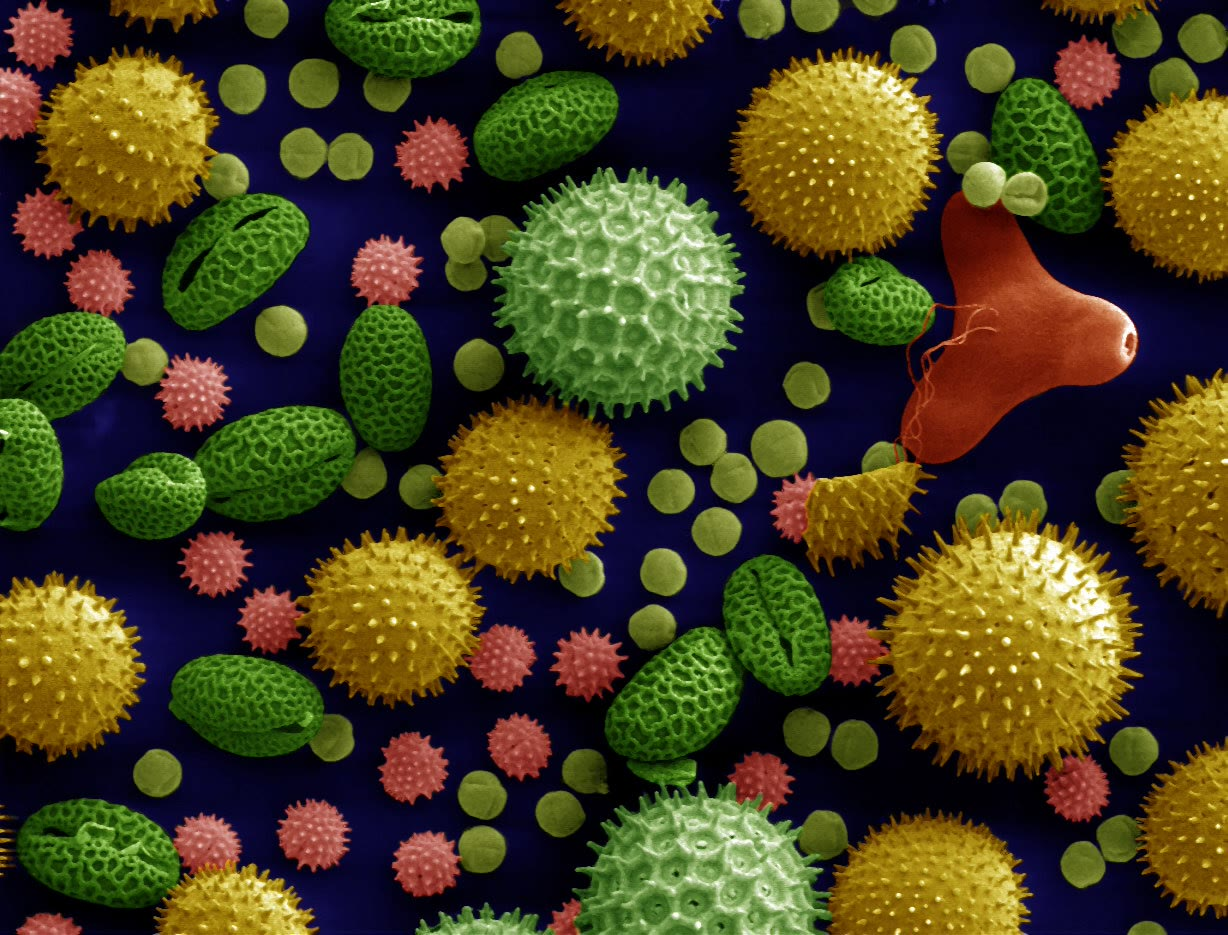
\includegraphics[width=0.46\linewidth]{images/book2/g12-pollen-sem.jpg}

{\small Granos de polen de cinco plantas comunes (girasol, campanilla,
malva real, lirio y prímula) vistos con un microscopio electrónico de barrido, en
falso color. Cada tipo de planta tiene su propia forma de grano. Dartmouth
Electron Microscope Facility (dominio público, vía Wikimedia Commons).}
\end{omfigure}
% ledger: photo:g12-pollen

\begin{definition}[Análisis polínico]\label{def:g12:past-climates:pollen}
El \emph{análisis polínico}\index{analisis polinico@análisis polínico} es la reconstrucción de la vegetación
del pasado a partir del polen conservado en los sedimentos: en cada capa de un testigo,
los granos se identifican y se cuentan, y la proporción de cada tipo de planta,
en porcentaje de los granos contados, se representa frente a la profundidad en un
\emph{diagrama polínico}\index{diagrama polinico@diagrama polínico}.
\end{definition}
% ledger: ncei:pollen

Contar el polen de este modo empezó con el geólogo sueco Lennart von
Post, que presentó el primer \omterm{def:g12:past-climates:pollen}{diagrama polínico} moderno, con cifras, en 1916;
un diagrama así muestra la profundidad hacia abajo de la página y una curva por cada tipo de
planta. La vegetación, a su vez, habla del clima: las gramíneas y otras
hierbas casi sin árboles indican un paisaje abierto y frío, mientras que el roble y el
avellano necesitan veranos cálidos.
% ledger: rull18:von-post; the Varden diagram is invented (ice_age_records.py POLLEN)

\begin{omfigure}
\begin{tikzpicture}
\pgfplotsset{pollen/.style={scale only axis, height=6cm, ymin=300, ymax=600,
  y dir=reverse, xmin=0, axis x line*=bottom, axis y line*=left, axis line style={-},
  tick label style={font=\scriptsize}, title style={font=\small, yshift=-4pt, text depth=0.25ex, text height=1.6ex},
  ytick={300,350,...,600}, xmajorgrids, ymajorgrids,
  grid style={gray!22, line width=0.3pt}}}
\begin{axis}[pollen, name=p1, width=3.0cm, xmax=100, xtick={0,20,...,80}, title={hierbas},
  ylabel={profundidad (cm)}, every axis label/.append style={font=\small}]
\addplot[fill=omLithSand, draw=black!70, line width=0.4pt] table[x=pct, y=depth_cm] {figdata/out/grade-12-ice_age_records-pol-herbs.dat};
\coordinate (z1) at (axis cs:0,550);
\coordinate (z2) at (axis cs:0,470);
\coordinate (z3) at (axis cs:0,425);
\end{axis}
\begin{axis}[pollen, name=p2, at={(p1.south east)}, anchor=south west, xshift=0.3cm,
  width=1.8cm, xmax=60, xtick={0,20,40}, title={abedul}, yticklabels={}]
\addplot[fill=omHypsLandB, draw=black!70, line width=0.4pt] table[x=pct, y=depth_cm] {figdata/out/grade-12-ice_age_records-pol-birch.dat};
\end{axis}
\begin{axis}[pollen, name=p3, at={(p2.south east)}, anchor=south west, xshift=0.3cm,
  width=1.8cm, xmax=60, xtick={0,20,40}, title={pino}, yticklabels={}]
\addplot[fill=omHypsLandA, draw=black!70, line width=0.4pt] table[x=pct, y=depth_cm] {figdata/out/grade-12-ice_age_records-pol-pine.dat};
\end{axis}
\begin{axis}[pollen, name=p4, at={(p3.south east)}, anchor=south west, xshift=0.3cm,
  width=1.2cm, xmax=40, xtick={0,20}, title={avellano}, yticklabels={}]
\addplot[fill=omHypsLandD, draw=black!70, line width=0.4pt] table[x=pct, y=depth_cm] {figdata/out/grade-12-ice_age_records-pol-hazel.dat};
\end{axis}
\begin{axis}[pollen, name=p5, at={(p4.south east)}, anchor=south west, xshift=0.3cm,
  width=1.5cm, xmax=50, xtick={0,20,40}, title={roble}, yticklabels={}]
\addplot[fill=omHypsLandE, draw=black!70, line width=0.4pt] table[x=pct, y=depth_cm] {figdata/out/grade-12-ice_age_records-pol-oak.dat};
\coordinate (e1) at (axis cs:50,550);
\coordinate (e2) at (axis cs:50,470);
\coordinate (e3) at (axis cs:50,425);
\coordinate (top) at (axis cs:50,300);
\coordinate (bot) at (axis cs:50,600);
\end{axis}
\draw[densely dashed, black!70] (z1) -- (e1 -| p5.east);
\draw[densely dashed, black!70] (z2) -- (e2 -| p5.east);
\draw[densely dashed, black!70] (z3) -- (e3 -| p5.east);
\node[font=\scriptsize, anchor=west] at ($(bot -| p5.east)!0.5!(e1 -| p5.east)$) {zona 1};
\node[font=\scriptsize, anchor=west] at ($(e1 -| p5.east)!0.5!(e2 -| p5.east)$) {zona 2};
\node[font=\scriptsize, anchor=west] at ($(e2 -| p5.east)!0.5!(e3 -| p5.east)$) {zona 3};
\node[font=\scriptsize, anchor=west] at ($(e3 -| p5.east)!0.5!(top -| p5.east)$) {zona 4};
\node[font=\scriptsize, anchor=north] at ($(p1.south)!0.5!(p5.south)+(0,-0.45)$) {porcentaje del polen contado};
\end{tikzpicture}

{\small Un \omterm{def:g12:past-climates:pollen}{diagrama polínico} de un lago de las Varden Hills, la región inventada
de esta serie: datos de ejercicio inventados, con la sucesión que se encuentra en muchos
lagos de la zona templada fría. El fondo del testigo (\qty{600}{cm}) tiene
\num{14000} años, y lo alto de la parte representada (\qty{300}{cm}), \num{6000} años,
con un ritmo de depósito constante entre ambos.}
\end{omfigure}
% invented exercise data (ice_age_records.py POLLEN); no ledger row

\begin{method}[Leer un diagrama polínico]
\begin{enumerate}
  \item Lee el eje vertical: la profundidad, con las capas más antiguas abajo;
        convierte las profundidades en edades con las dataciones del testigo.
  \item Para cada capa, busca las plantas con las mayores proporciones.
  \item Divide el testigo en zonas, cada una con su propio conjunto de plantas
        dominantes; sitúa los límites donde las curvas cambian más deprisa.
  \item Nombra la vegetación de cada zona (hierbas abiertas, bosque claro de abedules, bosque
        de pinos, bosque de frondosas) y el clima que necesita.
  \item Lee las zonas de abajo arriba como una historia del paisaje.
\end{enumerate}
\end{method}

En el diagrama de arriba, la zona 1 es un paisaje de hierbas, con algunos abedules: el
país abierto y frío que dejó el hielo. En la zona 2 se extiende primero el abedul, un árbol
resistente; el pino lo sigue en la zona 3; y en la zona 4 el avellano y el roble, que necesitan veranos
cálidos, toman el relevo. Leído de abajo arriba, el testigo cuenta el final del
\omterm{def:g12:past-climates:glacial-cycle}{periodo glacial} y la llegada del calor del \omterm{def:g12:past-climates:glacial-cycle}{interglacial}, a medida que el
bosque volvía a ocupar el terreno.

\section{Los sedimentos oceánicos y el ritmo astronómico}

En el fondo del océano abierto, el lodo se acumula lentamente y sin interrupción,
capa sobre capa, durante millones de años. Está lleno de conchas de
foraminíferos: organismos unicelulares cuya concha, de una fracción de
milímetro, suele ser de calcita. Unos flotan cerca de la
superficie; otros viven en el fondo marino.
% ledger: ucmp:forams, lr04:stack (benthic), photo:g12-forams (planktic)

\begin{omfigure}
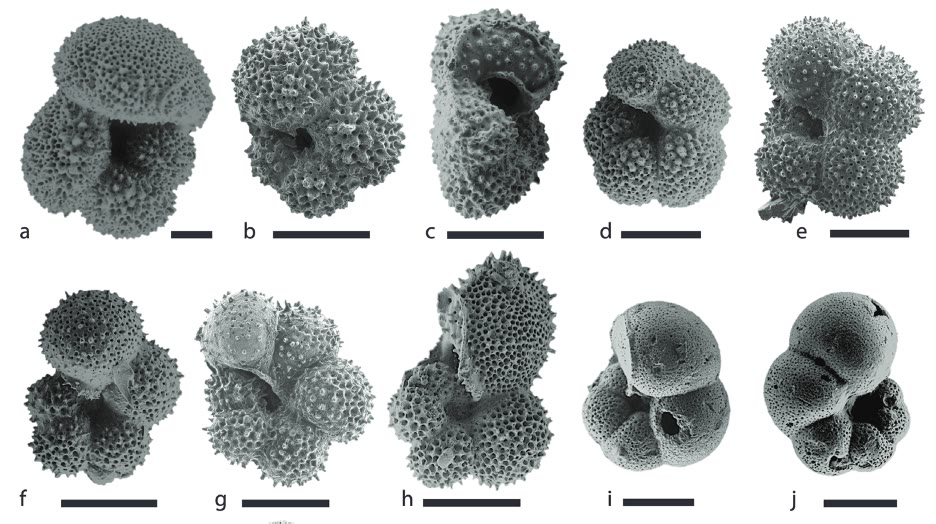
\includegraphics[width=0.62\linewidth]{images/book2/g12-planktic-foraminifera.jpg}

{\small Conchas de diez especies de foraminíferos que vivían flotando en el
océano, vistas con un microscopio electrónico de barrido; cada barra de escala mide
\qty{150}{\micro\metre}, así que cada concha tiene más o menos el tamaño de un grano de arena.
Marci Robinson, USGS (dominio público, vía Wikimedia Commons).}
\end{omfigure}
% ledger: photo:g12-forams

El oxígeno de una concha procede del agua del mar. El agua formada con el isótopo
ligero oxígeno 16 se evapora con más facilidad, y la nieve que construye los
inlandsis es por tanto pobre en oxígeno 18. Cuando los inlandsis crecen, almacenan
esta agua ligera, y el océano que queda se enriquece en oxígeno 18; lo
mismo les ocurre a las conchas que crecen en él, tanto más cuanto más fría está el agua. La proporción
de oxígeno 18 en las conchas de los foraminíferos del fondo marino, escrita
$\delta^{18}\mathrm{O}$ y expresada en partes por mil, es así un \omterm{def:g12:past-climates:proxy}{indicador indirecto} del
volumen de hielo sobre los continentes y de la temperatura del \omterm{def:g10:layered-ocean:thermocline}{océano profundo}: cuanto
más alta es, más hielo hay y más fría está el agua.
% ledger: nasaeo:o18, lr04:stack

El registro de abajo, llamado LR04, apila las medidas de 57 testigos de todos
los océanos en una sola curva de 5.3 millones de años.

\begin{omfigure}
\begin{tikzpicture}
\begin{axis}[omrecord, scale only axis, width=0.86\linewidth, height=4.8cm,
  xmin=0, xmax=5.32, x dir=reverse, ymin=2.4, ymax=5.3, y dir=reverse,
  xtick={0,0.5,...,5}, ytick={2.5,3,...,5},
  x tick label style={/pgf/number format/.cd, fixed, precision=1},
  y tick label style={/pgf/number format/.cd, fixed, fixed zerofill, precision=1},
  xlabel={millones de años antes de 1950},
  ylabel={$\delta^{18}\mathrm{O}$ de las conchas (\unit{\permil})}]
\fill[omProp!14] (axis cs:1.25,2.4) rectangle (axis cs:0.7,5.3);
% data:lr04 (the stack only; ice_age_records.py)
\addplot[omDef!85!black, line width=0.35pt] table[x=age_Ma, y=d18O] {figdata/out/grade-12-ice_age_records-lr04.dat};
\addplot[omThm, line width=1pt, densely dashed, unbounded coords=jump] table[x=age_Ma, y=d18O] {figdata/out/grade-12-ice_age_records-lr04mean.dat};
\coordinate (mpt) at (axis cs:0.975,2.45);
\coordinate (mm) at (axis cs:5.22,4.92);
\coordinate (arr) at (axis cs:5.12,3.9);
\end{axis}
\node[font=\scriptsize, anchor=north, align=center] at (mpt) {de 41 000 a\\100 000 años};
\draw[omThm, line width=1pt, densely dashed] (mm) -- ($(mm)+(0.5,0)$) node[right, font=\scriptsize, text=omThm] {medias de hace 5.3 a 3 y de 1 a 0 millones de años};
\draw[-{Stealth}, black!70] (arr) -- ++(0,-0.9) node[midway, right, font=\scriptsize, align=left] {más hielo,\\más frío};
\end{tikzpicture}

{\small Cinco millones de años del \omterm{def:g10:layered-ocean:thermocline}{océano profundo} en las conchas de los foraminíferos
del fondo marino; el eje vertical está invertido, para que las épocas frías y con mucho hielo queden
abajo. Las líneas discontinuas son las medias de la primera y la última parte. Sombreado:
el paso de un ritmo de \num{41000} años a otro de unos \num{100000}
años. Datos: Lisiecki y Raymo (2005), el apilamiento LR04.}
\end{omfigure}
% ledger: data:lr04, lr04:stack, clark06:mpt

Leído con el método anterior, el registro dice tres cosas.
\begin{itemize}
  \item \emph{La Tierra se ha enfriado y su hielo ha crecido.} El valor medio
        sube de \qty{3.03}{\permil} entre hace 5.3 y 3 millones de años
        a \qty{4.15}{\permil} en el último millón de años.
  \item \emph{Las oscilaciones han crecido.} Las épocas glaciales e \omterm{def:g12:past-climates:glacial-cycle}{interglaciales}
        se alternan a lo largo de todo el registro, pero oscilan cada vez más: en
        el \omterm{def:g12:past-climates:lgm}{Último Máximo Glacial} el valor era de \qty{4.92}{\permil}, frente a
        \qty{3.23}{\permil} hoy.
  \item \emph{El ritmo ha cambiado.} Entre hace 2.6 y 1.3 millones de años,
        el periodo más fuerte del registro, calculado a partir de sus datos, es de
        \num{41000} años; en los últimos \num{700000} años es de unos
        \num{98000} años, el ritmo de los \omterm{def:g12:past-climates:ice-core}{testigos de hielo}. El cambio tuvo
        lugar entre hace unos 1.25 y 0.7 millones de años.
\end{itemize}
% ledger: data:lr04, clark06:mpt (ice_age_records.py: lr04_mean_3_5Ma 3.032, lr04_mean_0_1Ma 4.147, lr04_lgm 4.92, lr04_today 3.23, periods 41.0 and 98.5 kyr)

Estos periodos no son casualidad. En 1976, James Hays, John Imbrie y Nicholas
Shackleton encontraron en los sedimentos de los océanos australes tres ritmos, de
\num{23000}, \num{42000} y unos \num{100000} años, que son los periodos
de cambios lentos de la órbita y del eje de la Tierra: la precesión del eje,
la inclinación del eje (unos \num{41000} años) y la forma de la órbita
(unos \num{100000} años). Estos cambios modifican la luz solar que recibe cada
latitud en cada estación, y marcan el paso de los \omterm{def:g12:past-climates:glacial-cycle}{ciclos
glaciales}. Cómo lo hacen, y por qué acabó imponiéndose el lento ritmo de \num{100000} años,
es materia de un curso universitario.
% ledger: hays76:periods, nasa:milankovitch, lr04:stack, clark06:mpt

\begin{dated}{2025}
En enero de 2025, el proyecto Beyond EPICA anunció que un testigo perforado en
Little Dome~C, a unos \qty{35}{km} de la estación Concordia, en el Domo~C, contiene
un registro continuo de hasta unos 1.2 millones de años en sus
\qty{2480}{m} superiores. Abarca la época
en que el ritmo glacial pasó de \num{41000} a \num{100000} años, y el
hielo y su aire se están analizando.
\end{dated}
% ledger: ku25:beyond-epica, ipev25:little-dome-c

\section{Los climas del tiempo profundo}

Más allá de lo que alcanzan los \omterm{def:g12:past-climates:ice-core}{testigos de hielo}, los climas del pasado se leen en los
sedimentos, las hojas y los suelos fósiles, y los isótopos. El IPCC ha elegido unos cuantos
\emph{periodos de referencia}, bien estudiados, cuyos climas ayudan a valorar
los cambios de hoy y de mañana. El gráfico de abajo da su temperatura media global
en superficie, respecto a 1850--1900.

\begin{omfigure}
\begin{tikzpicture}
\begin{axis}[omrecord, width=0.86\linewidth, height=5.4cm, xmin=-9, xmax=27,
  ymin=0.4, ymax=6.6, y dir=reverse, ytick={1,...,6}, ymajorgrids=false,
  yticklabels={{PETM, 56 Ma}, {EECO, 53--49 Ma}, {MPWP, 3.3--3.0 Ma},
    {LIG, 129--116 ka}, {LGM, 23--19 ka}, {MH, 6.5--5.5 ka}},
  y tick label style={font=\scriptsize},
  xlabel={temperatura respecto a 1850--1900 (\unit{\degreeCelsius})}]
% ipcc:fig2-34 (DEEP in ice_age_records.py)
\addplot[draw=none, mark=none, restrict expr to domain={\thisrow{tlo}}{0:30},
  error bars/.cd, x dir=both, x explicit,
  error bar style={line width=5pt, omWarm!75}, error mark=none]
  table[x expr={(\thisrow{tlo}+\thisrow{thi})/2}, y=idx,
        x error expr={(\thisrow{thi}-\thisrow{tlo})/2}] {figdata/out/grade-12-ice_age_records-deep.dat};
\addplot[draw=none, mark=none, restrict expr to domain={\thisrow{tlo}}{-30:-0.01},
  error bars/.cd, x dir=both, x explicit,
  error bar style={line width=5pt, omCold!75}, error mark=none]
  table[x expr={(\thisrow{tlo}+\thisrow{thi})/2}, y=idx,
        x error expr={(\thisrow{thi}-\thisrow{tlo})/2}] {figdata/out/grade-12-ice_age_records-deep.dat};
\draw[black!60] (axis cs:0,0.4) -- (axis cs:0,6.6);
\draw[omThm, densely dashed, line width=0.8pt] (axis cs:1.09,0.4) -- (axis cs:1.09,6.6);
\node[font=\scriptsize, text=omThm, anchor=west, fill=white, inner sep=1pt] at (axis cs:1.6,4.55) {2011--2020};
\end{axis}
\end{tikzpicture}

{\small Temperatura media global en superficie de seis periodos de referencia del pasado,
intervalos muy probables, respecto a 1850--1900; discontinua: la década 2011--2020.
Siglas en inglés del IPCC. PETM: Máximo Térmico del Paleoceno--Eoceno; EECO: Óptimo Climático
del Eoceno Temprano; MPWP: Periodo Cálido del Plioceno Medio; LIG: Último Interglacial; LGM: \omterm{def:g12:past-climates:lgm}{Último
Máximo Glacial}, el único frío (azul); MH:
Holoceno Medio. Valores: IPCC AR6 WG1, figura 2.34.}
\end{omfigure}
% ledger: ipcc:fig2-34, ipcc:gsat-2011-2020, ipcc:ref-periods

\begin{center}
\small
\begin{tabular}{|l|c|c|c|}
\hline
\textbf{periodo} & \textbf{temperatura (\unit{\degreeCelsius})} & \textbf{dióxido de carbono (ppm)} & \textbf{nivel del mar (m)} \\
\hline
PETM, 56 Ma & de $+10$ a $+25$ & unos 900, hasta 2000 & --- \\
EECO, 53--49 Ma & de $+10$ a $+18$ & de 1150 a 2500 & de $+70$ a $+76$ \\
MPWP, 3.3--3.0 Ma & de $+2.5$ a $+4.0$ & de 360 a 420 & de $+5$ a $+25$ \\
LIG, 129--116 ka & de $+0.5$ a $+1.5$ & de 266 a 282 & de $+5$ a $+10$ \\
\textcolor{omCold}{LGM, 23--19 ka} & \textcolor{omCold}{de $-7$ a $-5$} & \textcolor{omCold}{de 188 a 194} & \textcolor{omCold}{de $-134$ a $-125$} \\
MH, 6.5--5.5 ka & de $+0.2$ a $+1.0$ & de 260 a 268 & de $-3.5$ a $+0.5$ \\
\hline
\end{tabular}

\medskip
{\small Los periodos de referencia: temperatura media global en superficie respecto a
1850--1900, dióxido de carbono y nivel medio global del mar respecto a 1900. IPCC
AR6 WG1, figura 2.34.}
\end{center}
% ledger: ipcc:fig2-34

El Máximo Térmico del Paleoceno--Eoceno fue un calentamiento brusco, cuando un gran
pulso de carbono llegó al océano y al aire: el océano se volvió más ácido
y más pobre en oxígeno, y muchas especies de las profundidades marinas se extinguieron. En el Óptimo
Climático del Eoceno Temprano, el dióxido de carbono se mantuvo por encima de \qty{1000}{ppm} durante
millones de años, no había hielo polar, y bosques casi tropicales crecían
a \ang{70} de latitud sur. El Periodo Cálido del Plioceno Medio es la última vez que el dióxido
de carbono estuvo cerca del actual: el Ártico era mucho más cálido que ahora, y el mar
estaba más alto. En el Último Interglacial, los inlandsis de Groenlandia y de la Antártida
Occidental eran más pequeños y el mar más alto que hoy, y los hipopótamos vivían
en Gran Bretaña.
% ledger: ipcc:ref-periods, ipcc:fig2-34, ipcc:mpwp-eeco

Estos archivos sitúan el presente en perspectiva, y el propio IPCC hace la
comparación. En 2019, el dióxido de carbono del aire era más alto que en ningún otro momento de
al menos los últimos dos millones de años (\emph{confianza alta}), y los aumentos de dióxido
de carbono y de metano desde 1750 superan con mucho los cambios naturales entre \omterm{def:g12:past-climates:glacial-cycle}{periodos glaciales}
e \omterm{def:g12:past-climates:glacial-cycle}{interglaciales} de al menos los últimos \num{800000} años (\emph{confianza
muy alta}). La temperatura media global en superficie ha subido desde 1970 más deprisa que
en cualquier otro periodo de 50 años de al menos los últimos \num{2000} años
(\emph{confianza alta}). La década 2011--2020 fue más cálida que los siglos más cálidos
del \omterm{def:g12:past-climates:glacial-cycle}{interglacial} actual, hace unos \num{6500} años, y se acercó
al calor del Último Interglacial, hace unos \num{125000} años
(\emph{confianza media}).
% ledger: ipcc:co2-ch4-800kyr, ipcc:fastest-2000yr, ipcc:co2-2myr

También puede compararse la velocidad del cambio. De 1970 a 2025, la tendencia del
registro de la temperatura global es de \qty{0.20}{\degreeCelsius} por década, es decir,
unos \qty{20}{\degreeCelsius} por cada mil años si se mantuviera; el
calentamiento a la salida del último \omterm{def:g12:past-climates:glacial-cycle}{periodo glacial} fue de unos
\qty{0.86}{\degreeCelsius} por cada mil años de media. Las causas del cambio actual,
y en qué puede convertirse, son el tema del \cref{ch:g12:climate-change}.
% ledger: data:gistemp (ice_age_records.py: rate_1970_2025_C_per_decade 0.2012), ipcc:lgm-cooling, ipcc:ref-periods

\section{Ejercicios}

\begin{exercise}[$\star$]\label{exo:g12:past-climates:1}
Da el término: (a) una magnitud medida en un archivo que sustituye a una
variable climática no medida; (b) un cilindro de hielo extraído por perforación de un inlandsis;
(c) un intervalo cálido entre dos \omterm{def:g12:past-climates:glacial-cycle}{periodos glaciales}; (d) la reconstrucción de la
vegetación del pasado a partir del polen fósil; (e) el momento, hace unos \num{23000} a \num{19000}
años, en que los últimos inlandsis alcanzaron su mayor extensión.
\end{exercise}

\begin{exercise}[$\star$]\label{exo:g12:past-climates:2}
Para cada \omterm{def:g12:past-climates:proxy}{indicador indirecto}, nombra su archivo y aquello sobre lo que informa: (a) el aire de
las burbujas; (b) la proporción de polen de roble; (c) el oxígeno 18 de las conchas de los
foraminíferos del fondo marino; (d) la anchura de los anillos de los árboles.
\end{exercise}

\begin{exercise}[$\star$]\label{exo:g12:past-climates:3}
Durante la última transición deglacial, de hace unos \num{18000} a \num{11000}
años, el nivel del mar subió de unos \qty{-120}{m} a \qty{-50}{m}. (a) Calcula
el ritmo medio de subida, en milímetros por año. (b) De 2006 a 2018, el nivel del mar
subió \qty{3.7}{mm} al año. Compara.
\end{exercise}

\begin{exercise}[$\star$]\label{exo:g12:past-climates:4}
La temperatura global subió \qty{0.20}{\degreeCelsius} por década de
1970 a 2025. Expresa este ritmo por siglo y por cada mil años.
\end{exercise}

\begin{exercise}[$\star$]\label{exo:g12:past-climates:5}
Hays, Imbrie y Shackleton encontraron tres ritmos en los sedimentos oceánicos:
\num{23000}, \num{42000} y unos \num{100000} años. (a) Asocia cada uno con la
precesión del eje, la inclinación del eje y la forma de la órbita.
(b) ¿Cuántos ciclos de \num{41000} años caben en \num{1000000} años? ¿Y cuántos
ciclos de \num{100000} años?
\end{exercise}

\begin{exercise}[$\star\star$]\label{exo:g12:past-climates:6}
La recta de mínimos cuadrados del capítulo es $\mathrm{CO_2} \approx 266.6 +
7.83\,\Delta T$ (en ppm, con $\Delta T$ en \unit{\degreeCelsius}).
(a) Predice el dióxido de carbono para la temperatura media del \omterm{def:g12:past-climates:lgm}{Último Máximo
Glacial} en el Domo~C, \qty{-9.4}{\degreeCelsius}, y compáralo con los
\qty{190}{ppm} medidos. (b) Predícelo para el punto más cálido, \qty{+5.5}{\degreeCelsius},
y compáralo con el valor medido más alto, \qty{299}{ppm}. (c) Usa la recta
para estimar la temperatura del Domo~C que correspondería a \qty{427}{ppm}, el
valor de 2025 en Mauna Loa. ¿Por qué no está justificado este último uso de la recta?
\end{exercise}

\begin{exercise}[$\star\star$]\label{exo:g12:past-climates:7}
Usa el \omterm{def:g12:past-climates:pollen}{diagrama polínico} del lago de las Varden Hills. (a) ¿Cuál es el polen
dominante a \qty{580}{cm}, y qué paisaje indica? (b) La misma
pregunta a \qty{340}{cm}. (c) ¿Qué árbol se extiende primero después del frío, y
qué árboles llegan los últimos? (d) ¿Por qué podría la llegada de un árbol ir con retraso respecto al
calentamiento que la hizo posible?
\end{exercise}

\begin{exercise}[$\star\star$]\label{exo:g12:past-climates:8}
En el mismo testigo, el lodo a \qty{600}{cm} tiene \num{14000} años y el de
\qty{300}{cm}, \num{6000} años, con un ritmo de depósito constante.
(a) Calcula este ritmo en milímetros por año. (b) Halla la edad del límite
entre las zonas 2 y 3, a \qty{470}{cm}. (c) ¿Cuántos años representa una lámina
de \qty{1}{cm} de espesor?
\end{exercise}

\begin{exercise}[$\star\star$]\label{exo:g12:past-climates:9}
En el mapa del Sudeste Asiático, la tierra emergida pasa de 4.11 a
7.16 millones de kilómetros cuadrados cuando el mar baja \qty{130}{m}.
(a) Calcula la ganancia y su porcentaje. (b) En el mapa, un descenso de unos
\qty{36}{m} basta para unir Borneo con Asia. ¿Estuvo la isla unida durante todo el \omterm{def:g12:past-climates:lgm}{Último
Máximo Glacial}? Explícalo. (c) ¿Por qué la línea de costa del mapa es solo
aproximada?
\end{exercise}

\begin{exercise}[$\star\star$]\label{exo:g12:past-climates:10}
En el registro LR04, el valor en el \omterm{def:g12:past-climates:lgm}{Último Máximo Glacial} es de
\qty{4.92}{\permil} y el actual, de \qty{3.23}{\permil}. (a) ¿Cuál es el más alto,
y es lo que esperas? Explícalo con los inlandsis. (b) ¿Por qué se dibuja
invertido el eje vertical del registro?
\end{exercise}

\begin{exercise}[$\star\star$]\label{exo:g12:past-climates:11}
Un amigo dice: ``La correlación de 0.92 entre la temperatura antártica
y el dióxido de carbono demuestra que el dióxido de carbono controló las glaciaciones''.
(a) ¿Qué muestra una correlación, y qué no muestra? (b) Da otras dos
explicaciones que darían la misma correlación. (c) ¿Qué tipo de
información sobre los dos registros ayudaría a decidir?
\end{exercise}

\begin{exercise}[$\star\star\star$]\label{exo:g12:past-climates:12}
El periodo más fuerte del registro LR04 es de \num{41000} años entre hace 2.6
y 1.3 millones de años, y de \num{98500} años en los últimos \num{700000}
años. (a) ¿Cuántos ciclos contiene cada ventana? (b) ¿Qué cambio de la
órbita o del eje de la Tierra corresponde a cada periodo? (c) Explica por qué un registro con
una muestra cada \num{2000} años puede mostrar estos ritmos, pero no un cambio
que duró un siglo.
\end{exercise}

\begin{exercise}[$\star\star\star$]\label{exo:g12:past-climates:13}
El ritmo de aumento del dióxido de carbono fue de 192 a \qty{198}{ppm} por siglo en
1995--2014. Durante el Máximo Térmico del Paleoceno--Eoceno fue de 4 a
\qty{42}{ppm} por siglo, y durante la última transición deglacial, como mucho
unos \qty{10}{ppm} por siglo. (a) ¿Cuántas veces más rápido fue el aumento reciente
que el aumento más rápido de la última deglaciación? (b) ¿Y que las estimaciones más lenta y
más rápida del PETM? (c) El aumento del PETM fue de unos 900 a unos
\qty{2000}{ppm}. ¿Cuánto habría tardado a \qty{42}{ppm} por siglo,
y al ritmo actual?
\end{exercise}

\begin{exercise}[$\star\star\star$]\label{exo:g12:past-climates:14}
El IPCC estima que la temperatura global subió de 1 a
\qty{1.5}{\degreeCelsius} por cada mil años en la parte más rápida de la última
deglaciación, y que sobre Groenlandia subió unas diez veces más deprisa en los
siglos de calentamiento más rápido. (a) Da el ritmo de Groenlandia en
\unit{\degreeCelsius} por cada mil años y por década. (b) Compáralo con el
ritmo global actual de \qty{0.20}{\degreeCelsius} por década. (c) ¿Por qué no debe
compararse directamente un ritmo local con uno global?
\end{exercise}

\begin{exercise}[$\star\star\star$]\label{exo:g12:past-climates:15}
El nivel del mar estaba a unos \qty{-50}{m} hace \num{11000} años; supón que luego
subió a un ritmo constante de \qty{12}{m} por cada mil años, el ritmo medio de la deglaciación
principal. (a) ¿Cuándo pasó por \qty{-36}{m}, el nivel que une Borneo
con Asia en el mapa? (b) Después de ese momento, ¿podría una persona ir a pie de Borneo a
la península Malaya? (c) ¿Cuánto tardaría el mar en subir los últimos
\qty{36}{m}, si hubiera seguido a la misma velocidad?
\end{exercise}

\begin{problem}[{Problema de fin de semana --- 800 000 años de hielo antártico}]
\label{pb:g12:past-climates:1}
% ledger: data:edc-jouzel, data:co2-bereiter, data:lr04, data:gistemp, ipcc:lgm-cooling, ipcc:ref-periods, hays76:periods, clark06:mpt
% values (ice_age_records.py): edc -10.58 / +5.46, co2 173.71 / 298.6, r 0.9165, fit 266.57 + 7.827 T,
% LGM -9.389 / 189.67, 11-9 ka -0.360 / 264.10, period 97.5, rate 0.2012 per decade, ratio 23.48
El hielo del Domo~C y el aire de sus burbujas dan los valores siguientes. La
temperatura es el cambio sobre el hielo respecto a los últimos mil años.

\begin{center}
\small
\begin{tabular}{|l|c|c|}
\hline
 & \textbf{\shortstack{cambio de\\temperatura (\unit{\degreeCelsius})}} & \textbf{\shortstack{dióxido de\\carbono (ppm)}} \\
\hline
valor más frío, hace unos \num{24000} años & $-10.6$ & --- \\
valor más cálido, hace unos \num{129000} años & $+5.5$ & --- \\
dióxido de carbono más bajo y más alto & --- & 174 y 299 \\
media, de hace \num{23000} a \num{19000} años & $-9.4$ & 190 \\
media, de hace \num{11000} a \num{9000} años & $-0.4$ & 264 \\
\hline
\end{tabular}
\end{center}

El periodo más fuerte del registro de temperatura es de unos \num{98000} años,
y los 1639 pares de valores dan un coeficiente de correlación de 0.92.

\medskip
\noindent\textbf{Parte I --- Leer los dos registros.}
\begin{enumerate}
  \item ¿Qué parte del hielo registra la temperatura, y cuál registra el
        dióxido de carbono?
  \item Calcula la amplitud total del cambio de temperatura en el Domo~C.
  \item Calcula la amplitud total del dióxido de carbono.
  \item ¿Qué dice un coeficiente de correlación de 0.92 sobre los dos
        registros?
  \item En la figura con eje de tiempo del capítulo, el presente está a la derecha. ¿Por qué
        debes comprobar en qué sentido corre el tiempo antes de leer una figura así?
\end{enumerate}

\medskip
\noindent\textbf{Parte II --- Valores glaciales e interglaciales.}
\begin{enumerate}[resume]
  \item Define un \omterm{def:g12:past-climates:glacial-cycle}{periodo glacial} y un \omterm{def:g12:past-climates:glacial-cycle}{interglacial}.
  \item ¿En cuál de los dos vivimos, y desde cuándo?
  \item ¿Cuántos ciclos de \num{98000} años caben en \num{800000} años?
  \item ¿Qué cambio de la órbita de la Tierra tiene un periodo cercano a
        \num{100000} años?
  \item Antes de hace unos 1.25 millones de años, ¿cuál era el ritmo principal de
        los \omterm{def:g12:past-climates:glacial-cycle}{ciclos glaciales}?
\end{enumerate}

\medskip
\noindent\textbf{Parte III --- La última deglaciación.}
\begin{enumerate}[resume]
  \item ¿Cuánto subió la temperatura sobre el Domo~C entre el \omterm{def:g12:past-climates:lgm}{Último
        Máximo Glacial} y el intervalo de hace \num{11000} a \num{9000} años?
  \item ¿Cuánto subió el dióxido de carbono en el mismo intervalo?
  \item La temperatura global del \omterm{def:g12:past-climates:lgm}{Último Máximo Glacial} era de 5 a
        \qty{7}{\degreeCelsius} inferior a la de 1850--1900. Toma el centro de
        este intervalo. ¿Es mayor o menor el cambio antártico?
  \item La última transición deglacial duró de hace \num{18000} a
        \num{11000} años. ¿Cuánto tiempo es eso?
  \item Calcula el ritmo medio del calentamiento global durante la transición, en
        \unit{\degreeCelsius} por cada mil años.
  \item Expresa este ritmo en \unit{\degreeCelsius} por década.
\end{enumerate}

\medskip
\noindent\textbf{Parte IV --- El ritmo actual, en comparación.}
\begin{enumerate}[resume]
  \item De 1970 a 2025, la temperatura global subió
        \qty{0.20}{\degreeCelsius} por década. Expresa este ritmo por
        cada mil años.
  \item ¿Cuántas veces más rápido es el calentamiento actual que el calentamiento medio de
        la última deglaciación?
  \item En la parte más rápida de la deglaciación, la temperatura global subió
        de 1 a \qty{1.5}{\degreeCelsius} por cada mil años. ¿Cuántas veces
        más rápido es el ritmo actual que estos?
  \item Concluye: ¿cuántas veces más rápido que el calentamiento a la salida de la última
        glaciación es el calentamiento global actual?
\end{enumerate}
\end{problem}
